%------------------------------------------------
% main.tex - test file for camel.cls
%------------------------------------------------
\documentclass{camel}
\usepackage{camel}

\academicyear{2014-15}
\modulecode{MA0000}
\moduletitle{Test Module}
\booktitle{Lecture Notes}

\usepackage{graphicx}

%----------------------------------------------------------------------
\begin{document}
\makefrontmatter
%----------------------------------------------------------------------

%----------------------------------------------------------------------
\chapter{Theorems}\label{ch:theorems}
%----------------------------------------------------------------------

Here is an equation with a label:
\begin{equation}\label{eq:einstein}
E = mc^2
\end{equation}

Here is a theorem:
\begin{theorem}\label{thm:euler}
$e^{i\pi}-1=0$.
\end{theorem}
\begin{proof}
TODO
\end{proof}

Here is a lemma:
\begin{lemma}\label{lem:zorn}
If a partially ordered set $A$ has the property that every totally ordered subset has an upper bound in $A$, then $A$ contains at least one maximal element.
\end{lemma}
\begin{proof}
TODO
\end{proof}


%----------------------------------------------------------------------
\chapter{Figures}\label{ch:figures}
%----------------------------------------------------------------------

Here is a figure.
\begin{figure}[htb]
\centering
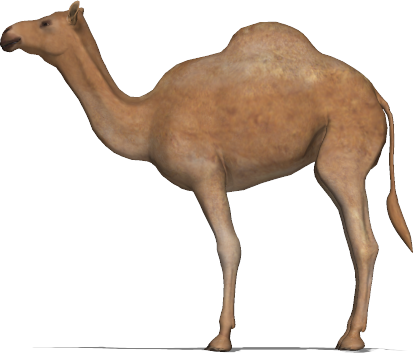
\includegraphics[scale=0.25]{figures/humpty.png}
\caption{Humpty the Camel.}
\label{humpty-the-camel}
\end{figure}

No more figures.

%----------------------------------------------------------------------
\chapter{Lists}\label{ch:lists}
%----------------------------------------------------------------------

Initial text.
\begin{itemize}
\item First item of list
\begin{enumerate}
\item First item of nested list.
\item Second item of nested list.
\end{enumerate}
\item Second item of list
\end{itemize}
Final text.

%----------------------------------------------------------------------
\chapter{Labels, References and Citations}
%----------------------------------------------------------------------

\begin{itemize}
\item Here we include a label: \label{ch:introduction}.
\item Here we include a reference: \ref{ch:introduction}.
\item Here we include a citation: \cite{video_ex.1.1.1}.
\end{itemize}

%----------------------------------------------------------------------
\chapter{Exercises}\label{ch:exercises}
%----------------------------------------------------------------------

%---------------------------------------
\section{Formative exercises}
%---------------------------------------
\begin{formative}\label{fex:demo}
This is the introduction.
\begin{questions} 
\question This is the first question.\label{qu:fex:demo:first-question}
\begin{answer} 
This is the answer to the first question.
\end{answer} 
\question This is the second question.\label{qu:fex:demo:second-question}
\begin{answer} 
This is the answer to the second question.
\end{answer} 
\question This is the third question.\label{qu:fex:demo:third-question}
\begin{parts}
\part This is the first part of the third question
\begin{answer} 
This is the answer to the first part of the third question.
\end{answer} 
\part This is the second part of the third question
\begin{answer} 
This is the answer to the second part of the third question.
\end{answer} 
\end{parts}
\end{questions} 
\end{formative}

%---------------------------------------
\section{Diagnostic exercises (multiple choice}
%---------------------------------------
\begin{diagnostic}\label{dex:demo} 
\begin{questions} 
\question Which is the odd one out? \label{qu:dex:demo:first-question}
\begin{choices} 
\correctchoice Mick
\choice Paul 
\choice George 
\choice Ringo 
\end{choices} 
\question Which is the odd one out? \label{qu:dex:demo:second-question} 
\begin{choices} 
\choice John 
\correctchoice Keef 
\choice George 
\choice Ringo 
\end{choices} 
\end{questions}
\end{diagnostic}


\end{document}

